\begin{ledgroupsized}[r]{120mm}
\footnotesize 
\pstart 
\noindent\textbf{\"{U}berlieferung:}
\pend
\end{ledgroupsized}
\begin{ledgroupsized}[r]{114mm}
\footnotesize 
\pstart \parindent -6mm
\makebox[6mm][l]{\textit{L}}%
Konzept: LH XXXV 10, 9 Bl. 3-4. 1 Bog. 2\textsuperscript{o}. 1\,\nicefrac{1}{3} Sp. auf Bl.~3~r\textsuperscript{o}.
Der Bogen überliefert ferner N.~28\textsubscript{1}, N.~28\textsubscript{2}, N.~28\textsubscript{6} und N.~5.
%LH35,10,09 Bl. 3r = Demonstratio geometrica de magnetis sphaera
\\
Cc 2, Nr. 1191 (tlw.)
\pend
\end{ledgroupsized}

%%\normalsize
%\vspace*{5mm}
%\begin{ledgroup}
%\footnotesize 
%\pstart
%\noindent\footnotesize{\textbf{Datierungsgr\"{u}nde}: bisher keine absolute Datierung, nur Einordnung in Sequenz zur Kraft am Rad erfolgt}
%\pend
%\end{ledgroup}
 
\vspace*{8mm}
\count\Bfootins=1200
\count\Cfootins=1200
\pstart 
\normalsize
\noindent[3~r\textsuperscript{o}]\edtext{}{\lemma{\hspace{1.8mm}[\textit{Fig. 1}]}\killnumber\Cfootnote{Die Parallele \textit{ATR} ist gestrichen. \hspace{7cm}}} Centro $L$ esto \edtext{circulus $LN$ intervalla $LQ$ diametri}{\lemma{circulus $LN$} \Bfootnote{\textit{(1)}\ intervalla $LP$ in radio item alia minora \textit{(2)}\ intervalla $LQ$ \textit{(a)}\ in circul \textit{(b)}\ diametri \textit{L}}} portiones inter se aequales $AB$, $AB \hspace{0.5mm}\sqcap\hspace{0.5mm} TS\hspace{0.5mm} \sqcap \hspace{0.5mm}\beta$ tangens respondens intercepta: $NMO$ vel $RGS$. Sit triangulum $STR$, ducatur $TE$ parallela $LG$ erit ang. $GLF\hspace{1mm} \sqcap$ angulo $ETS$. Ergo ang. $TSR \, \sqcap \, \text{angulo} \, FGL$. Ergo $RS$ ad $TS$ seu $RS$ \edtext{ad $\beta$ ut $LG \sqcap a$ ad}{\lemma{ad $\beta$}\Bfootnote{ \textit{(1)}\ ut $a$ ad \textit{(2)}\ ut $LG \sqcap a$ ad \textit{ L}}} $FG \sqcap y$ et erit \rule[-4mm]{0mm}{10mm}$RS \sqcap \displaystyle\frac{a \beta}{y}$.
\pend
\vspace{1em}
\pstart
\noindent
%\begin{wrapfigure}[14]{l}{0.42\textwidth}
%\vspace{-5mm}
\setline{6}\centering
\includegraphics[trim = 0mm -2mm 0mm 0mm, clip, width=0.4\textwidth]{images/lh0351009_003r_2-d2.pdf}\\
\noindent \centering [\textit{Fig. 1}] 
%\end{wrapfigure}
\pend
\pstart Itaque vis ponderis\protect\index{Sachverzeichnis}{vis ponderis} descendentis in circuli circumferentia, erit ad vim ejusdem ponderis descendentem recta, in ratione $\beta$ ad \rule[-4mm]{0mm}{10mm}$\displaystyle\frac{a \beta}{y}$ sive ut $y$ ad $a$, sive ut sinus ad \rule[-4mm]{0mm}{10mm}\edtext{radium, et pone $LQ \hspace{1mm} \sqcap \hspace{1mm}\displaystyle\frac{a^2}{b}$ erit vis ponderis in $LQ \hspace{1mm}\sqcap \hspace{1mm}\displaystyle\frac{y}{b}$. Jam}{\lemma{radium,} \Bfootnote{\textit{(1)}\ pone jam $a \sqcap 1$. \textit{(2)}\ et pone $LQ \sqcap \displaystyle\frac{a^2}{b}$ erit vis ponderis in $LQ \sqcap \displaystyle\frac{y}{b}$. Jam \textit{L}}}\rule[-4mm]{0mm}{10mm} cum duae sint $y$, una $\sqcap \hspace{1mm}DM$ altera $\sqcap \hspace{1mm}LG$ quarum puncta $M.\ G$ quadrante distant, relatione quadam perpetua explicandae rectae $DM$, et $LG$, quae aequatione quadam sive regula exprimatur. Nimirum recta $MG$ est data et constans $\surd{2a^2}$ seu $a\surd{2}$. 
\pend 
\pstart Datur $LG \sqcap a$. Ponamus $LF \sqcap x$ et $FG \sqcap z$. Fiet: $a^2-x^2 \sqcap z^2$. Porro datur \edtext{$DM \sqcap y$}{\lemma{$DM \sqcap y$}\Cfootnote{Hiermit $y$ neu gesetzt. Vorher galt: $FG \sqcap y$.}} et $DL \rule[-4mm]{0mm}{10mm} \sqcap \sqrt{a^2 - y^2}$ ergo $DF$ sive $MK \sqcap \sqrt{a^2 - y^2} + x$ et $KG^2 \sqcap \ovalbox{2} a^2 \ovalbox{$-a^2$} -y^2 -x^2 -2x \sqrt{a^2 - y^2}$.\edtext{}{\lemma{$KG^2$ [...] $-2x \sqrt{a^2 - y^2}$}\Cfootnote{Korrekter Wert für $KG^2$ ist $y^2$. Den Fehler berichtigt die Gleichung $z\, \sqcap\, (\alpha \omega \alpha \omega) \sqrt{y^6 - y^4 + y^2 + 1} (\omega \omega \alpha \alpha) \displaystyle\frac{y^3}{a^2}$ auf S.~\pageref{LH0351009_003r_Gleichung}.}} 
\pend
\vspace{1.5em}
\pstart
\begin{center}                    
\setline{6}\includegraphics[width=0.5\textwidth]{images/lh0351009_003r_2-d4.pdf}\\
\end{center}
\noindent \centering [\textit{Fig. 2}]
\pend
\newpage
\pstart \noindent Et fiet: seu \rule[-4mm]{0mm}{10mm}$KG \sqcap \displaystyle\efrac{\sqrt{+a^2 - x^2 - 2x \sqrt{a^2 - y^2}}}{-y^2\hfill}$ et $FG$ erit \rule[-4mm]{0mm}{10mm}$\sqcap \displaystyle\efrac{\sqrt{a^2 - x^2 - 2x \sqrt{a^2 - y^2}}}{-y^2\hfill} (\PsMs) y \sqcap z$ sive \rule[-4mm]{0mm}{10mm}$\displaystyle\efrac{+a^2 - x^2 - 2 \sqrt{a^2 - y^2} x}{-y^2 \hfill}\sqcap z^2 (\MsPs) 2yz + y^2$ sive $a^2-y^2$ appellando per compendium $\omega^2$, fiet: \rule[-4mm]{0mm}{10mm}\edtext{aequatio}{\lemma{fiet:} \Bfootnote{\textit{(1)}\ $\omega^2-x^2-2\omega$ \textit{(2)}\ aequatio \textit{L}}} $\displaystyle\efrac{z^2 + x^2 (\MsPs) 2yz + 2\omega x - a^2}{\hfill +2y^2}\sqcap 0$. Jam supra $z^2x^2-a^2 \sqcap 0$. Ergo conferendo posteriorem ex priore, fiet: $(\MsPs) \cancel{2}yz + \cancel{2}\omega x + \cancel{2}y^2 \sqcap 0$. \edtext{Ideoque}{\lemma{$\cancel{2}y^2 \sqcap 0$}\Bfootnote{\textit{(1)} sive $z\sqcap \displaystyle\frac{\cancel{2}\omega x + \cancel{2}y^2}{\cancel{2}y}$ \textit{(2)} Ideoque \textit{ L}}} $x\sqcap \displaystyle\frac{\MsPs \hspace{0.5mm} yz - y^2}{\omega}$\rule[-4mm]{0mm}{10mm} et \rule[-4mm]{0mm}{10mm}$x^2\sqcap \displaystyle\frac{-y^2 z^2 (\PsMs) 2y^3 z+y^4}{a^2 - y^2}$ \rule[-4mm]{0mm}{10mm}quem valorem substituendo in aequatione $z^2+x^2-a^2 \sqcap 0$ fiet: $z^2 a^2 \ovalbox{$-z^2y^2, +y^2z^2$} (\PsMs) 2y^3z + y^4, -a^4 - y^2 a^2 \sqcap 0$\edtext{}{\lemma{$- y^2 a^2$}\Cfootnote{Das Vorzeichen des Terms muss positiv sein.}} \edtext{fingendo}{\lemma{}\Bfootnote{fingendo \textit{erg. L}}} $y^4-a^2y^2-a^4$, \rule[-4mm]{0mm}{10mm}ea aequatio \edtext{ficta}{\lemma{}\Bfootnote{ficta \textit{erg. L}}} nullum habet divisorem. Divisores enim ejus: $a.\ a^2.\ a^3$ atqui aequatio haec dividi potest neque per $y \hspace{1mm} \PsMs \hspace{1mm} a$, neque per $y^2 \hspace{1mm}\PsMs \hspace{1mm} a^2$, neque per $y^3 \hspace{1mm}\PsMs \hspace{1mm} a^3$. Nam $y$ et $a$, idem $y^3$ et $a^3$ excluduntur, ponendo literas pro \edtext{quadratis, quia}{\lemma{quadratis,}\Bfootnote{\textit{(1)}\ quas \textit{(2)}\ quia \textit{L}}} nullae aliae adsunt: restat ergo
\begin{minipage}[t]{0.2\textwidth}
\begin{tabular}{r}
$y^2 \hspace{1mm}\PsMs \hspace{1mm}a^2$\\
$y^2 + ca$\\
$y^4 + cay^2 \hspace{1mm}\PsMs\hspace{1mm} ca^3$\\
$\PsMs \hspace{1mm}a^2 \cdot \cdot \hspace{8mm}$\\
\end{tabular}
\end{minipage}
Videamus. Multiplicemus per $-y^2 \hspace{1mm}\PsMs \hspace{1mm} ca$ et conferendo: fiet $-a \sqcap \PsMs \hspace{0.5mm} c$, sive $c \sqcap \MsPs \hspace{0.5mm} a$ et rursus conferendo: \edtext{$\MsPs \hspace{0.5mm} a^2 \hspace{1mm}\PsMs \hspace{1mm} a^2 \sqcap -a^2$}{\lemma{$\MsPs \hspace{0.5mm} a^2 \hspace{1mm}\PsMs\hspace{1mm}  a^2 \sqcap -a^2$}\Cfootnote{Der erste Term heißt eigentlich $ca$ statt $a^2$.}}, quod est \protect\rule[-4mm]{0mm}{8mm}absurdum. Divisio ergo non procedit: ergo erit \rule[-4mm]{0mm}{10mm}\edtext{$z^2 \hspace{1mm}(\PsMs) \hspace{1mm} \displaystyle\frac{2y^3}{a^2}z+ \protect\rule[-4mm]{0mm}{10mm}\displaystyle\frac{y^6}{a^4} \sqcap \displaystyle\frac{\sqrt{y^6 - y^4a^2 + y^2a^4 + a^6}}{a^4}$}{\lemma{$\displaystyle\frac{\sqrt{y^6 - y^4a^2 + y^2a^4 + a^6}}{a^4}$}\Cfootnote{Das Vorzeichen des Terms $y^2a^4$ muss negativ sein. Der Fehler wirkt sich auf die folgenden Ableitungen aus.}} $\PsPsMs \hspace{0.5mm} z\hspace{1mm} \PsMsPs\hspace{1mm}  \protect\rule[-4mm]{0mm}{10mm}\displaystyle\frac{y^3}{a^2} \sqcap \displaystyle\frac{\sqrt{y^6 - y^4a^2 + y^2a^4 + a^6}}{a^2}$ sive $z \sqcap \displaystyle\frac{\PsPsMs \hspace{0.5mm}\sqrt{y^6 - y^4a^2 + y^2a^4 + a^6}\hspace{1mm} (\MsPs)\hspace{1mm} y^3}{a^2}$\rule[-4mm]{0mm}{10mm}.
 \pend 
 \count\Bfootins=1500
\count\Cfootins=1500
 \pstart
Ergo si $a \sqcap 1$ erit $z \sqcap \PsPsMs \hspace{0.5mm} \sqrt{y^6 - y^4 + y^2 + 1} (\MsPs) y^3$ \\
\begin{minipage}[t]{0.1\textwidth}
\begin{tabular}{ll} 
$\alpha$ & $\alpha$\\
$\omega$ & $\omega$\\
$\alpha$ & $\omega$\\
$\omega$ & $\alpha$\\
\end{tabular} \\
\end{minipage}
$(\alpha \omega \alpha \omega) z (\alpha \omega \omega \alpha) \displaystyle\frac{y^3}{a^2} \sqcap \sqrt{\dots}$ unde $z + (\alpha \alpha \omega \omega) \displaystyle\frac{y^3}{a}\sqcap \sqrt{\dots}$\\ sive\setline{5} $z \sqcap (\alpha \omega \alpha \omega) \sqrt{y^6 - y^4 + y^2 + 1} (\omega \omega \alpha \alpha) \displaystyle\frac{y^3}{a^2}$\rule[-4mm]{0mm}{10mm}.\label{LH0351009_003r_Gleichung} 
\pend 
%\newpage
\pstart%
Sed \setline{6}post calculum satis
\edtext{prolixum, exactius excuti}{\lemma{prolixum}\Bfootnote{\textit{(1)}\ et forte alicubi erroneum \textit{(2)}\ exactius excuti \textit{L}}}
dignum, Geometria\protect\index{Sachverzeichnis}{geometria} facillimam exhibet constructionem pariter et construendi rationem ope angulorum.
Nam Triangula $LFG$, $MDL$ similia sunt, quod ita ostendo.
Angulus $PLG$ rectus ex constructione et angulus $DLM\, \sqcap\, \text{angulo}\ PLF.$ ergo angulus $DML\, \sqcap\, \text{angulo}\ GLF$.
Triangula ergo quae dixi similia sunt.
Habent autem unum latus aequale $LM$ et $LG$ ob circulum.
Ergo Triangula $LFG.$ $MDL$ non tantum similia sed et aequalia erunt.
Ergo erit $FG \sqcap DL$, et $DM \sqcap LF$.
%
Ergo ponendo $DM \sqcap y$ erit\rule[-4mm]{0mm}{10mm}
$\edtext{[FG]}{\lemma{$FM$}\Bfootnote{\textit{L ändert Hrsg.}}}
\sqcap \sqrt{a^2 - y^2}$
erit ergo semper \rule[-4mm]{0mm}{10mm}$\displaystyle\frac{agy + g \sqrt{1 - y^2}}{b} - gy\
\edtext{\lbrack-\rbrack}{\lemma{$+$}\Bfootnote{\textit{L ändert Hrsg.}}}
g \sqrt{1 - y^2}
\ \sqcap\
%
\edtext{\displaystyle\frac{agy + ag \sqrt{1 - y^2} - bgy\
\edtext{\lbrack-\rbrack}{\lemma{$+$}\Bfootnote{\textit{L ändert Hrsg.}}}
bg \sqrt{1 - y^2}}{ba}$%
\edtext{.
%
%
Sive $\displaystyle\efrac{}{((} \displaystyle\frac{ay + a \sqrt{a^2 - y^2},}{b} - \displaystyle\frac{y + \sqrt{1 - y^2}}{a} \displaystyle\efrac{}{))}\smallfrown \displaystyle\frac{g}{a}$.%
}{\lemma{$\displaystyle\frac{agy + ag \sqrt{1 - y^2} - bgy\ \lbrack-\rbrack bg \sqrt{1 - y^2}}{ba}$ %
[...] $\smallfrown \displaystyle\frac{g}{a}$}%
\Cfootnote{Leibniz rechnet mit $a = 1$.}}
%
Unde ponendo $y \sqcap 1$}{%
\lemma{$\displaystyle\frac{agy + ag \sqrt{1 - y^2} - bgy\ \lbrack-\rbrack bg \sqrt{1 - y^2}}{ba}$}%
\Bfootnote{\textit{(1)}\ ponendo jam $y \sqcap 1$ \textit{(2)}. Sive [...] $y \sqcap 1$ \textit{ L}}}
%
seu machina\protect\index{Sachverzeichnis}{machina} in situ perpendiculari posita, fiet:
\rule[-4mm]{0mm}{10mm}$y - \displaystyle\frac{y}{b}, \smallfrown g$.
Ponendo $y\, \sqcap\, \displaystyle\frac{1}{2}.$ quando scilicet $DLM$ angulus est 30 graduum, fiet:
%
$\ovalbox{$\displaystyle\frac{1}{2}$ + \ovalbox{$\sqrt{1 - \displaystyle\frac{1}{4}}$} $\displaystyle\frac{\sqrt3}{2}$}\ \ \displaystyle\frac{1 + \sqrt3}{2} - \displaystyle\frac{1 + \sqrt3}{2b}$.
Pone $b\ \text{esse}\, \sqcap\, 10$, tunc posito
\edtext{$y\, \sqcap\, 1$ vis erit:}{\lemma{$y\, \sqcap\, 1$}%
\Bfootnote{\textit{(1)} \textbar\ fiet: \textit{streicht Hrsg.}\ \textbar\ vis agens\ \textit{(2)} vis erit: \textit{ L}}}
%
$\displaystyle\frac{10 - 1}{10} \sqcap \displaystyle\frac{9}{10} g$.
Ponendo $y\, \sqcap \displaystyle\frac{1}{2}$,
fiet:\rule[-4mm]{0mm}{10mm} $\displaystyle\frac{10 + 10 \sqrt3 - 1 - \sqrt3}{20}$ sive $\displaystyle\frac{9 + 9 \sqrt3}{20}$ etc. 
\pend%
\newpage
\pstart%
Regula ergo haec est: ab $y + \sqrt{1 - y^2}$
\edtext{auferatur ab eodem idem diviso}{\lemma{auferatur}\Bfootnote{\textit{(1)}\ $y+\sqrt{}$ idem divisum \textit{(2)}\ ab eodem idem diviso \textit{L}}}
per $b$.
Residuum multiplicetur per \rule[-4mm]{0mm}{10mm}$\displaystyle\frac{g}{a}$ factus erit
\edtext{vis machinae}{\lemma{vis}\Bfootnote{\textit{(1)}\ ponderis \textit{(2)}\ machinae \textit{L}}}.
Ponendo Vim absolutam\protect\index{Sachverzeichnis}{vis absoluta ponderis} ponderis unius exigui esse $g$\rule[-4mm]{0mm}{6mm}
multiplicatam per radium $1$ et $b$ esse quantitatem radii minoris,
seu distantiam ponderis\protect\index{Sachverzeichnis}{pondus} \setline{6}centro propioris. 
\pend
%\pstart Sed post calculum satis \edtext{prolixum, exactius excuti}{\lemma{prolixum}\Bfootnote{\textit{(1)}\ et forte alicubi erroneum \textit{(2)}\ exactius excuti \textit{L}}} dignum, Geometria\protect\index{Sachverzeichnis}{geometria} facillimam exhibet constructionem pariter et construendi rationem ope angulorum. Nam Triangula $LFG$, $MDL$ similia sunt, quod ita ostendo. Angulus $PLG$ rectus ex constructione et angulus $DLM \sqcap \text{angulo}\ PLF$ ergo angulus $DML \sqcap \text{angulo}\ GLF$. Triangula ergo quae dixi similia sunt. Habent autem unum latus aequale $LM$ et $LG$ ob circulum. Ergo Triangula $LFG$ $MDL$ non tantum similia sed et aequalia erunt. Ergo erit $FG \sqcap DL$, et $DM \sqcap LF$. Ergo ponendo $DM \sqcap y$ \edtext{erit $FG \sqcap \sqrt{a^2 - y^2}$}{\lemma{$FG \sqcap \sqrt{a^2 - y^2}$} \Cfootnote{Leibniz schreibt f\"{a}lschlicherweise $FM$ anstelle von $FG$.}} erit ergo semper \rule[-4mm]{0mm}{10mm}$\displaystyle\frac{agy + g \sqrt{1 - y^2}}{b} - gy + g \sqrt{1 - y^2} \sqcap \displaystyle\frac{agy + ag \sqrt{1 - y^2} - bgy + bg \sqrt{1 - y^2}}{ya}$. \rule[-4mm]{0mm}{10mm}\edtext{Sive $\displaystyle\efrac{}{((} \displaystyle\frac{ay + a \sqrt{a^2 - y^2},}{b} - \displaystyle\frac{y + \sqrt{1 - y^2}}{a} \displaystyle\efrac{}{))}\smallfrown \displaystyle\frac{g}{a}$. Unde ponendo $y \sqcap 1$}{\lemma{$\sqcap \displaystyle\frac{agy + ag \sqrt{1 - y^2} - bgy + bg \sqrt{1 - y^2}}{ba}$}\Bfootnote{\textit{(1)}\ ponendo jam $y \sqcap 1$. \textit{(2)} sive $\displaystyle\efrac{}{((} \displaystyle\frac{ay + a \sqrt{a^2 - y^2},}{b} - \displaystyle\frac{y + \sqrt{1 - y^2}}{a} \displaystyle\efrac{}{))}\!\smallfrown \displaystyle\frac{g}{a}$. Unde ponendo $y \sqcap 1$ \textit{ L}}} seu machina\protect\index{Sachverzeichnis}{machina} in situ perpendiculari posito, fiet: \rule[-4mm]{0mm}{10mm}$y - \displaystyle\frac{y}{b}, \smallfrown g$. Ponendo $y \sqcap \displaystyle\frac{1}{2}$ quando scilicet $DLM$ angulus est 30 graduum, fiet: \\
%$\ovalbox{$\displaystyle\frac{1}{2}$ + \ovalbox{$\sqrt{1 - \displaystyle\frac{1}{4}}$} $\displaystyle\frac{\sqrt3}{2}$} \quad \displaystyle\frac{1 + \sqrt3}{2} - \displaystyle\frac{1 + \sqrt3}{2b}$. Pone $b\ \text{esse} \sqcap 10$, tunc posito $y \sqcap 1$ fiet: vis erit: \\
%$\displaystyle\frac{10 - 1}{10} \sqcap \displaystyle\frac{9}{10} g$. Ponendo $y \sqcap \displaystyle\frac{1}{2}$, fiet:\rule[-4mm]{0mm}{10mm} $\displaystyle\frac{10 + 10 \sqrt3 - 1 - \sqrt3}{20}$ sive $\displaystyle\frac{9 + 9 \sqrt3}{20}$ etc. 
%\pend 
%\pstart Regula ergo haec est: ab $y + \sqrt{1 - y^2}$ auferatur \edtext{ab eodem idem diviso}{\lemma{auferatur} \Bfootnote{\textit{(1)}\ $y+\sqrt{}$ idem divisum \textit{(2)}\ ab eodem idem diviso \textit{L}}} per $b$. Residuum multiplicetur per \rule[-4mm]{0mm}{10mm}$\displaystyle\frac{g}{a}$ factus erit vis \edtext{machinae}{\lemma{vis} \Bfootnote{\textit{(1)}\ ponderis \textit{(2)}\ machinae \textit{L}}}. Ponendo Vim absolutam\protect\index{Sachverzeichnis}{vis absoluta ponderis} ponderis unius exigui esse $g$ multiplicatam per radium $1$ et $b$ esse quantitatem radii minoris, seu distantiam ponderis\protect\index{Sachverzeichnis}{pondus} centro propioris. 
%\pend 
%\vspace{1em}
%\newpage
\vspace{2em}
\pstart\noindent
%\begin{wrapfigure}[4]{l}{0.35\textwidth}
%\vspace{-3mm}
\centering
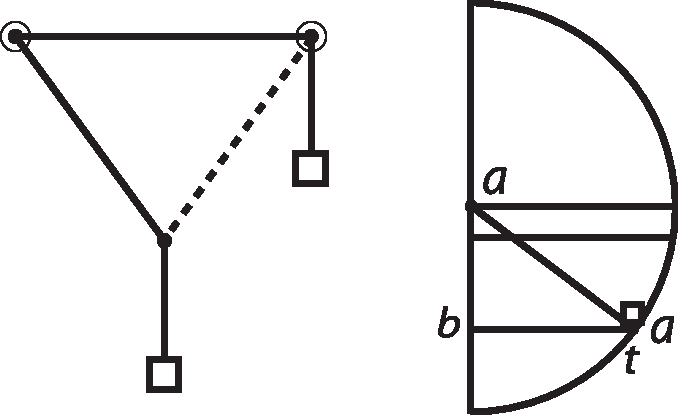
\includegraphics[trim = 0mm -5mm 0mm 0mm, clip, width=0.35\textwidth]{images//lh0351009_003r_2-d5+6.pdf}\\
\noindent \centering [\textit{Fig. 3 und Fig. 4 gestr.}]
%\end{wrapfigure}\\
%\includegraphics[width=0.2\textwidth]{images/lh0351009_003r_2-d5.pdf}
%\hspace{10mm} 
%\includegraphics[width=0.15\textwidth]{images/lh0351009_003r_2-d6.pdf}\\
%\vspace{8mm}
\pend
\vspace{2em}
\pstart
\noindent [\textit{Nachfolgend \setline{5}kleingedruckter Text gestrichen}:]
\pend
\vspace{0.5em}
\pstart
\noindent
\footnotesize
{Comme $b$ est \`{a} $a$, ainsi la force du poids\protect\index{Sachverzeichnis}{force du poids} descendant dans la} \edtext{\small{[circonference]}}{\lemma{}\Bfootnote{circomference \textit{L }\textit{\"{a}ndert Hrsg.}}} \small{du cercle, du point $ab$, est [\textit{Text bricht ab}.]} 
\pend
\count\Bfootins=1200
\count\Cfootins=1200